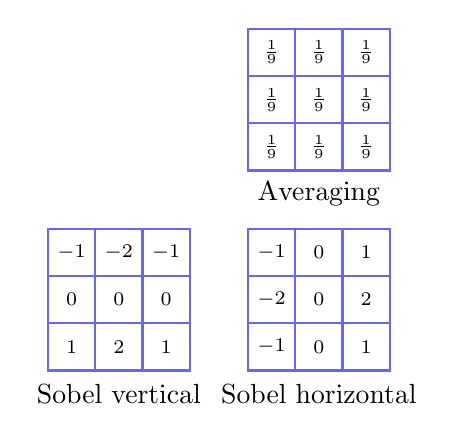
\begin{tikzpicture}[x=0.6cm, y=0.6cm]
%Ranga Rodrigo
%September 11, 2019


\def\rows{6}
\def\cols{7}
\def\linecol{blue!60}

\begin{filecontents*}{./sobelv.dat}
-1
-2
-1
0
0
0
1
2
1
\end{filecontents*}


\begin{filecontents*}{./sobelh.dat}
-1
0
1
-2
0
2
-1
0
1
\end{filecontents*}


\begin{scope}[xshift=1in]
% Kernel only
\draw[thick, \linecol] (0,0) rectangle ++(3,3);
\draw[thick, \linecol] (0,1) rectangle ++(3,1);
\draw[thick, \linecol] (1,0) rectangle ++(1,3);

\foreach \i in {0,1,2}
{
	\foreach \j in {0,1,2}
	{
		\node at (\i + 0.5, \j + 0.5) {\scriptsize $\frac{1}{9}$};
	}
}
\node at (1.5, -0.5) {Averaging};
\end{scope}

\begin{scope}[yshift=-1in]
% Kernel only
\draw[thick, \linecol] (0,0) rectangle ++(3,3);
\draw[thick, \linecol] (0,1) rectangle ++(3,1);
\draw[thick, \linecol] (1,0) rectangle ++(1,3);

\pgfplotstableread{./sobelv.dat}{\sobelvs}
	
	\foreach \i in {0,1, 2}
	{
		\foreach \j in {0,1, 2}
		{	
			\pgfmathsetmacro{\index}{\i*3+\j}%
			\pgfplotstablegetelem{\index}{[index] 0}\of{\sobelvs}%
			\let\sobelv\pgfplotsretval%
			\node at (\j + 0.5, 2.5 - \i) {\scriptsize $\sobelv$};
	}
}
\node at (1.5, -0.5) {Sobel vertical};
\end{scope}

\begin{scope}[xshift=1in, yshift=-1in]
% Kernel only
\draw[thick, \linecol] (0,0) rectangle ++(3,3);
\draw[thick, \linecol] (0,1) rectangle ++(3,1);
\draw[thick, \linecol] (1,0) rectangle ++(1,3);

\pgfplotstableread{./sobelh.dat}{\sobelhs}
	
	\foreach \i in {0,1, 2}
	{
		\foreach \j in {0,1, 2}
		{	
			\pgfmathsetmacro{\index}{\i*3+\j}%
			\pgfplotstablegetelem{\index}{[index] 0}\of{\sobelhs}%
			\let\sobelh\pgfplotsretval%
			\node at (\j + 0.5, 2.5 - \i) {\scriptsize $\sobelh$};
	}
}
\node at (1.5, -0.5) {Sobel horizontal};
\end{scope}


\end{tikzpicture}
